\section{Architektur}
\label{sec:architektur}

\subsection{Gesamtarchitektur}

SignalReport folgt einer monolithischen Architektur, bei der alle Komponenten in einer
einzigen JAR-Datei zusammengefasst sind. Diese Entscheidung wurde bewusst getroffen, um
die Installation so einfach wie möglich zu halten -- es wird kein separater
Datenbankserver, kein Application-Server und kein Build-System beim Endbenutzer benötigt.

Das Deployment-Diagramm in Abbildung \ref{fig:deployment} zeigt die drei Ebenen der
Architektur: den Client (Browser), das Server-System (JVM mit allen Komponenten) und die
externen Dienste (DNS-Server, Web-Server, ipify.org).

\begin{figure}[H]
    \centering
    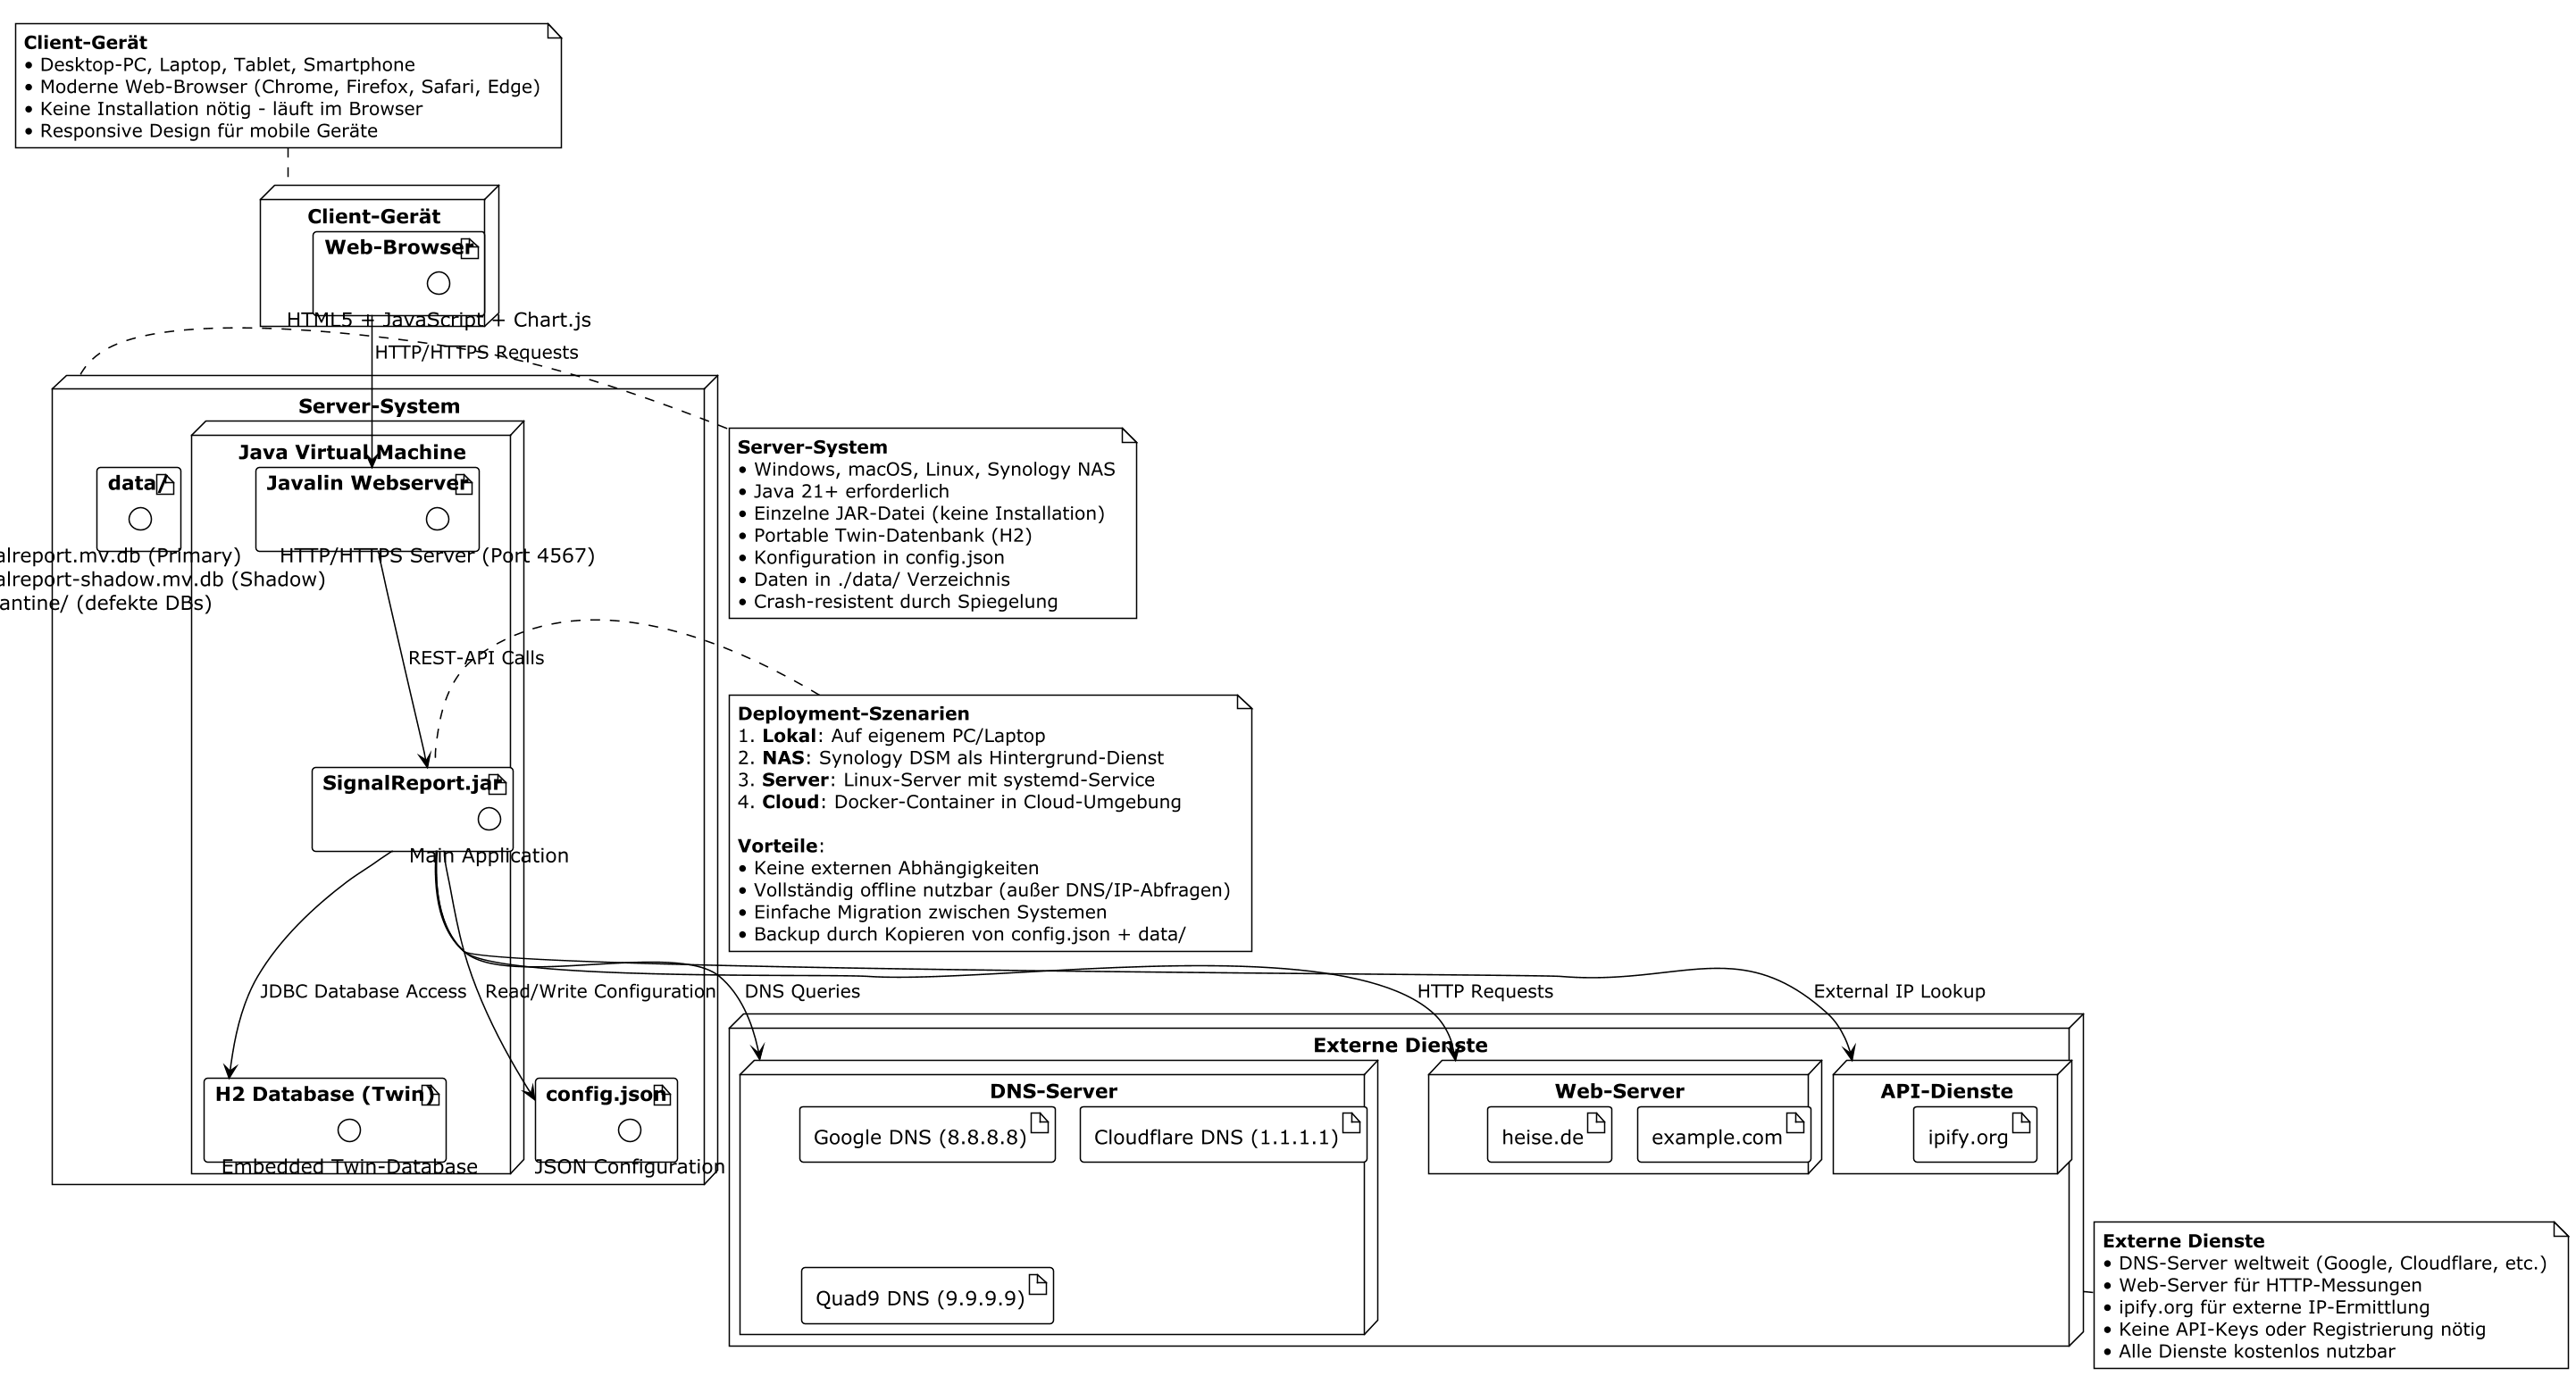
\includegraphics[width=\textwidth]{../diagrams/deployment-diagram.png}
    \caption{Deployment-Diagramm von SignalReport}
    \label{fig:deployment}
\end{figure}

\subsection{Komponenten-Design}

Die Anwendung gliedert sich in sieben Haupt-Packages (Abbildung \ref{fig:component}):

\begin{description}
  \item[measurement] Mess-Engine mit dem \texttt{Measurer}-Interface und drei
    Implementierungen (Ping, DNS, HTTP) sowie dem DNS-Benchmark.
  \item[model] Das \texttt{Measurement}-Datenobjekt als zentrales Transferobjekt.
  \item[persistence] \texttt{H2MeasurementRepository} für die embedded Datenbank
    in Twin-Architektur (Primary + Shadow). Tabellen: Messungen, Hosts, IP-Änderungen.
    Siehe Abschnitt \ref{subsec:twindb}.
  \item[config] Singleton-Konfiguration mit JSON-Persistenz und verschachtelten
    Konfigurations-Klassen (Targets, MaintenanceWindow, Auth, Theme, etc.).
  \item[web] \texttt{WebServer} (Javalin) mit ausgelagertem HTML-Rendering in
    \texttt{HtmlPageRenderer}, \texttt{SetupPageRenderer} und
    \texttt{LoginPageRenderer}. Session-Verwaltung und
    Challenge-Response-Verifikation über \texttt{SessionManager}.
  \item[export] \texttt{PdfReportGenerator} (OpenPDF + JFreeChart) und
    \texttt{PushNotificationService} für Browser-Benachrichtigungen.
  \item[network] \texttt{HostIdentifier} (stabiler Host-Hash) und \texttt{NetworkInfo}
    (lokale/externe IP-Ermittlung).
\end{description}

\begin{figure}[H]
    \centering
    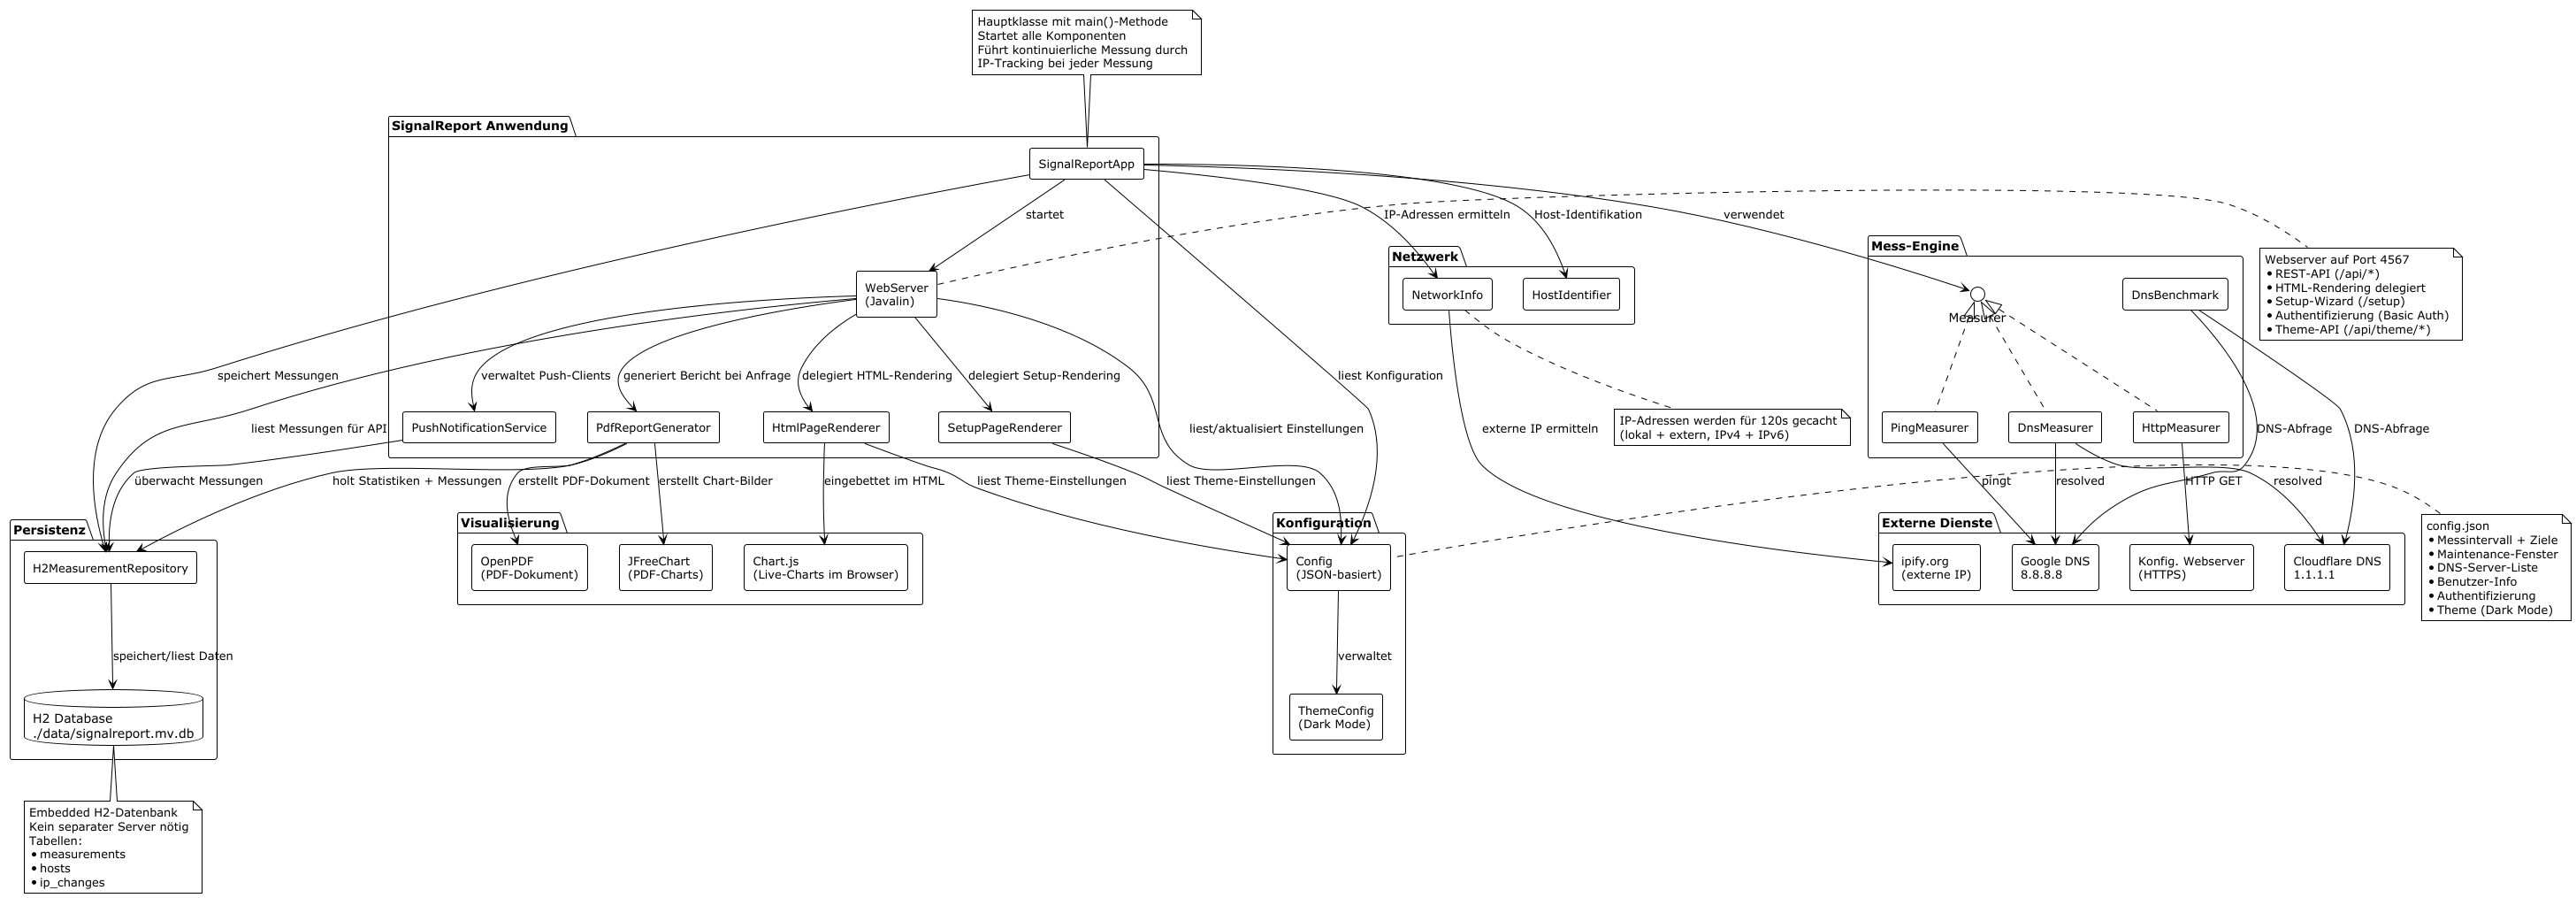
\includegraphics[width=\textwidth]{../diagrams/component-diagram.png}
    \caption{Komponenten-Übersicht von SignalReport}
    \label{fig:component}
\end{figure}

\subsection{Klassen-Design}

Das Klassen-Diagramm in Abbildung \ref{fig:class} zeigt die vollständige Klassenstruktur.
Besonders hervorzuheben sind:

\begin{itemize}
  \item Das \textbf{Measurer-Interface} (Strategy-Pattern): Alle drei Messtypen
    implementieren das gleiche Interface \texttt{Measurer} mit der Methode
    \texttt{measure(String target)}. Dadurch können neue Messtypen hinzugefügt werden,
    ohne bestehenden Code zu ändern (Open/Closed Principle).
  \item Die \textbf{Renderer-Klassen}: Das HTML-Rendering wurde aus dem WebServer in
    eigenständige Klassen ausgelagert (\texttt{HtmlPageRenderer},
    \texttt{SetupPageRenderer}), um die Trennung von Verantwortlichkeiten (Separation of
    Concerns) zu wahren. Der WebServer schrumpfte dadurch von über 2100 auf ca.\ 800
    Zeilen.
  \item Die \textbf{Config-Hierarchie}: Verschachtelte statische Klassen für verschiedene
    Konfigurationsbereiche; zentrale \texttt{hashPassword()}-Methode statt dupliziertem Code.
\end{itemize}

\begin{figure}[H]
    \centering
    
\includegraphics[width=\textwidth]{../diagrams/class-diagram.png}
    \caption{Klassen-Diagramm von SignalReport}
    \label{fig:class}
\end{figure}

\subsection{Design-Entscheidungen}

\begin{table}[h]
\centering
\begin{tabular}{|l|p{9cm}|}
\hline
\textbf{Entscheidung} & \textbf{Begründung} \\
\hline
Monolithische Architektur & Einfachste Installation: eine JAR-Datei, keine externen
  Abhängigkeiten \\
\hline
H2 Embedded Database & Plattformunabhängig, kein separater DB-Server, portable
  Datei \\
\hline
Twin-DB-Architektur & Synchrone Spiegelung in zweite H2-Datei; bei Korruption
  wird die intakte Kopie automatisch zur Reparatur verwendet (vgl.\ Abschnitt \ref{subsec:twindb}) \\
\hline
Javalin statt Spring Boot & Minimaler Overhead (ca.\ 5\,MB vs.\ 30+\,MB), schneller
  Startup \\
\hline
Java 21 & Virtual Threads, Pattern Matching, Text Blocks fuer
  HTML-Templates \\
\hline
OpenPDF statt PDFBox & Einfachere API für Tabellen und Charts; bessere
  Schriftarten-Unterstützung \\
\hline
Inline-HTML statt Templates & Kein Template-Engine-Overhead; Java Text Blocks ermöglichen
  lesbaren HTML-Code; Dark Mode via CSS Custom Properties \\
\hline
Apache Commons Daemon & Professioneller Dienst-Betrieb auf allen Plattformen
  (procrun/jsvc) \\
\hline
\end{tabular}
\caption{Architektur-Entscheidungen (Architecture Decision Records)}
\label{tab:adr}
\end{table}

\subsection{Twin-Datenbank-Architektur}
\label{subsec:twindb}

Nach der Diplomprüfung trat im Produktivbetrieb ein Korruptionsfall der H2-Datenbank
auf, ausgelöst durch einen unvermittelten Windows-Update-Neustart genau während eines
Schreibvorgangs. Die \texttt{.mv.db}-Datei war anschließend nicht mehr lesbar, und auch
das offizielle H2-Recovery-Tool konnte keinen einzigen konsistenten Chunk mehr finden.
Die historischen Messdaten waren damit unwiederbringlich verloren.

Daraufhin wurde die Persistenzschicht von einer einzelnen H2-Datenbank auf eine
\textbf{Twin-Architektur} mit zwei parallel geführten H2-Dateien umgestellt:

\begin{itemize}
  \item \textbf{Primary} (\texttt{signalreport.mv.db}): autoritative Quelle für alle
    Lese-Operationen.
  \item \textbf{Shadow} (\texttt{signalreport-shadow.mv.db}): synchrone Spiegelung
    aller Schreiboperationen.
\end{itemize}

Jede Schreiboperation (\texttt{save}, \texttt{registerHost}, \texttt{recordIpChange})
wird über einen zentralen \texttt{writeOnBoth(\dots)}-Helper sequenziell auf beide
Connections angewendet -- zuerst auf die Primary, danach auf die Shadow. Lese-Operationen
gehen ausschließlich auf die Primary, was den Performance-Overhead minimiert.

\paragraph{Schutz-Stufen.} Drei zusammenwirkende Mechanismen sorgen für Robustheit
gegen abrupte Prozess-Terminierungen (Stromausfall, Update-Neustart, kill -9):

\begin{enumerate}
  \item \texttt{WRITE\_DELAY=0} im JDBC-URL: Jede Transaktion wird synchron auf die
    Platte geflusht (statt Default 500\,ms). Damit verkleinert sich das Korruptions-Fenster
    von Hunderten von Millisekunden auf wenige Mikrosekunden.
  \item \textbf{Twin-Spiegelung}: Selbst wenn eine der beiden Dateien während eines
    Schreibvorgangs zerstört wird, bleibt die jeweils andere konsistent.
  \item \textbf{Auto-Recovery beim Start}: Erkennt der Konstruktor von
    \texttt{H2MeasurementRepository} eine Korruption (H2-Fehlercode 90030), wird die
    defekte Datei in ein \texttt{quarantine/}-Unterverzeichnis verschoben und per
    \texttt{Files.copy()} aus der intakten DB rekonstruiert. Anschließend werden beide
    Connections normal geöffnet -- der Betrieb läuft unterbrechungsfrei weiter.
\end{enumerate}

\paragraph{Fehlerszenarien.} Die Tabelle \ref{tab:twindb-szenarien} dokumentiert das
Verhalten bei den verschiedenen Krisenfällen:

\begin{table}[H]
\centering
\begin{tabular}{|p{5cm}|p{9cm}|}
\hline
\textbf{Szenario} & \textbf{Verhalten} \\
\hline
Crash während Primary-Write & Primary korrupt, Shadow intakt $\to$
  Beim Neustart wird die Primary aus der Shadow rekonstruiert; maximaler Datenverlust:
  die Schreibvorgänge der letzten Sekunden auf die Shadow \\
\hline
Crash während Shadow-Write & Shadow korrupt, Primary intakt $\to$
  Beim Neustart wird die Shadow aus der Primary rekonstruiert; kein Datenverlust \\
\hline
Beide DBs korrupt & Extrem unwahrscheinlich (erfordert Filesystem-Schaden) $\to$
  Beide Dateien werden in Quarantäne verschoben, Betrieb startet mit leeren
  Datenbanken neu, Anwendung bleibt funktional \\
\hline
Shadow-Korruption zur Laufzeit & Sehr selten; Shadow wird deaktiviert, Primary
  läuft weiter, beim nächsten Neustart wird die Shadow automatisch repariert \\
\hline
\end{tabular}
\caption{Twin-DB-Verhalten bei Korruptionsfällen}
\label{tab:twindb-szenarien}
\end{table}

\paragraph{Migration bestehender Installationen.} Existiert beim Update auf die neue
Version bereits eine alte Single-DB ohne Shadow, wird im ersten Konstruktor-Aufruf
die Shadow als exakte Kopie der Primary angelegt. Damit greift die Twin-Redundanz
sofort -- ohne Datenverlust und ohne manuelle Migrationsschritte.

\subsection{Internationalisierung (i18n)}
\label{subsec:i18n}

Die gesamte Präsentationsschicht -- Web-Oberfläche, Login- und Setup-Seite,
PDF-Berichte, CSV-Spaltenköpfe und benutzerseitige API-Meldungen -- ist
mehrsprachig. Aktuell werden neun Sprachen mitgeliefert: Deutsch (Referenz),
Englisch, Französisch, Italienisch, Spanisch, Portugiesisch, Türkisch, Polnisch
und Ukrainisch.

\paragraph{Sprachdateien.} Jede Sprache ist eine flache JSON-Datei (UTF-8) mit
Punkt-Schlüsseln unter \texttt{resources/lang/}, z.\,B.
\texttt{"nav.settings": "Einstellungen"}. Die zentrale Klasse \texttt{I18n}
lädt die in der Konfiguration hinterlegte Sprache und stellt drei Mechanismen
bereit:

\begin{enumerate}
  \item \textbf{Platzhalter-Auflösung}: Die HTML-Renderer enthalten statt
    deutscher Literale Platzhalter der Form \texttt{\{\{nav.settings\}\}}.
    \texttt{I18n.resolve()} ersetzt sie beim Rendern per regulärem Ausdruck.
  \item \textbf{JS-Injektion}: Texte, die das Frontend-JavaScript zur Laufzeit
    erzeugt (Status-Badges, Chart-Beschriftungen, Fehlermeldungen), werden als
    \texttt{const I18N = \{...\}}-Objekt in die Seite eingebettet. Datums- und
    Zahlenformate folgen über die mitgereichte Locale der gewählten Sprache.
  \item \textbf{Direkte Aufrufe}: PDF-Generator und WebServer verwenden
    \texttt{I18n.get(key)} sowie locale-bewusste Formatierung
    (\texttt{String.format(locale, ...)}) -- im Deutschen erscheint
    \texttt{23,5 ms}, im Englischen \texttt{23.5 ms}.
\end{enumerate}

\paragraph{Fallback-Kette.} Fehlt ein Schlüssel in der gewählten Sprache, wird
auf Deutsch (Referenzsprache) zurückgegriffen, danach auf den Schlüsselnamen
selbst -- die Oberfläche zeigt also nie ein Loch. Ein eigener Testfall
(\texttt{I18nTest}) erzwingt zusätzlich, dass alle mitgelieferten Sprachdateien
exakt dieselben Schlüssel wie die Referenz enthalten und dass jeder im
Quellcode verwendete Platzhalter existiert.

\paragraph{Erweiterbarkeit ohne Neukompilieren.} Neben den im JAR gebündelten
Sprachen liest \texttt{I18n} einen externen Ordner \texttt{./lang} neben der
JAR-Datei ein. Eine dort abgelegte Datei (z.\,B. \texttt{ca.json} für
Katalanisch) erscheint automatisch im Sprach-Dropdown; gleichnamige Dateien
überschreiben gebündelte Sprachen, womit auch Übersetzungskorrekturen ohne
Neubau möglich sind. Der Anzeigename jeder Sprache stammt aus ihrem eigenen
Schlüssel \texttt{language.name} und erscheint im Dropdown in der jeweiligen
Eigenbezeichnung (Deutsch, English, Türkçe, Ukrainisch in kyrillischer
Schrift usw.).

\paragraph{Sprachwahl.} Die Sprache wird global pro Installation in
\texttt{config.json} gespeichert. Sie ist an zwei Stellen umstellbar: per
Dropdown im Setup-Wizard (noch vor der Passwortvergabe, via
\texttt{/setup?lang=xx}) und im Einstellungen-Tab (sofortige Übernahme über
\texttt{POST /api/config/language} mit anschließendem Seiten-Reload).
Neuinstallationen starten in der Systemsprache des Rechners, sofern
unterstützt -- andernfalls auf Englisch. Bestehende Konfigurationen ohne
\texttt{language}-Feld bleiben unverändert auf Deutsch.

\paragraph{PDF und Sonderzeichen.} Die eingebauten PDF-Schriften (Helvetica)
beherrschen nur Westeuropa-Zeichen; Türkisch, Polnisch und Ukrainisch wären
damit im Bericht nicht darstellbar. Deshalb wird die freie Schrift
\textbf{DejaVu Sans} (Regular, Bold, Oblique) als Ressource mitgeliefert und
mit Unicode-Encoding (\texttt{IDENTITY\_H}) in jedes PDF eingebettet. Dieselben
TTF-Dateien dienen JFreeChart als AWT-Schrift, sodass auch Chart-Titel und
Achsenbeschriftungen in allen Sprachen korrekt gerendert werden. Der
JAR-Zuwachs durch Schriften und neun Sprachdateien beträgt rund 1,5\,MB.

\subsection{Datenfluss bei der Messung}

Der Messablauf (Abbildung \ref{fig:sequence-measurement}) zeigt den kontinuierlichen
Zyklus:
\begin{enumerate}
  \item Konfiguration laden und Maintenance-Fenster prüfen
  \item Externe IP ermitteln und IP-Änderungen protokollieren
  \item Drei Messungen ausführen (Ping, DNS, HTTP)
  \item Ergebnisse in der Datenbank speichern
  \item Konfigurierbares Intervall abwarten
\end{enumerate}

\begin{figure}[H]
    \centering
    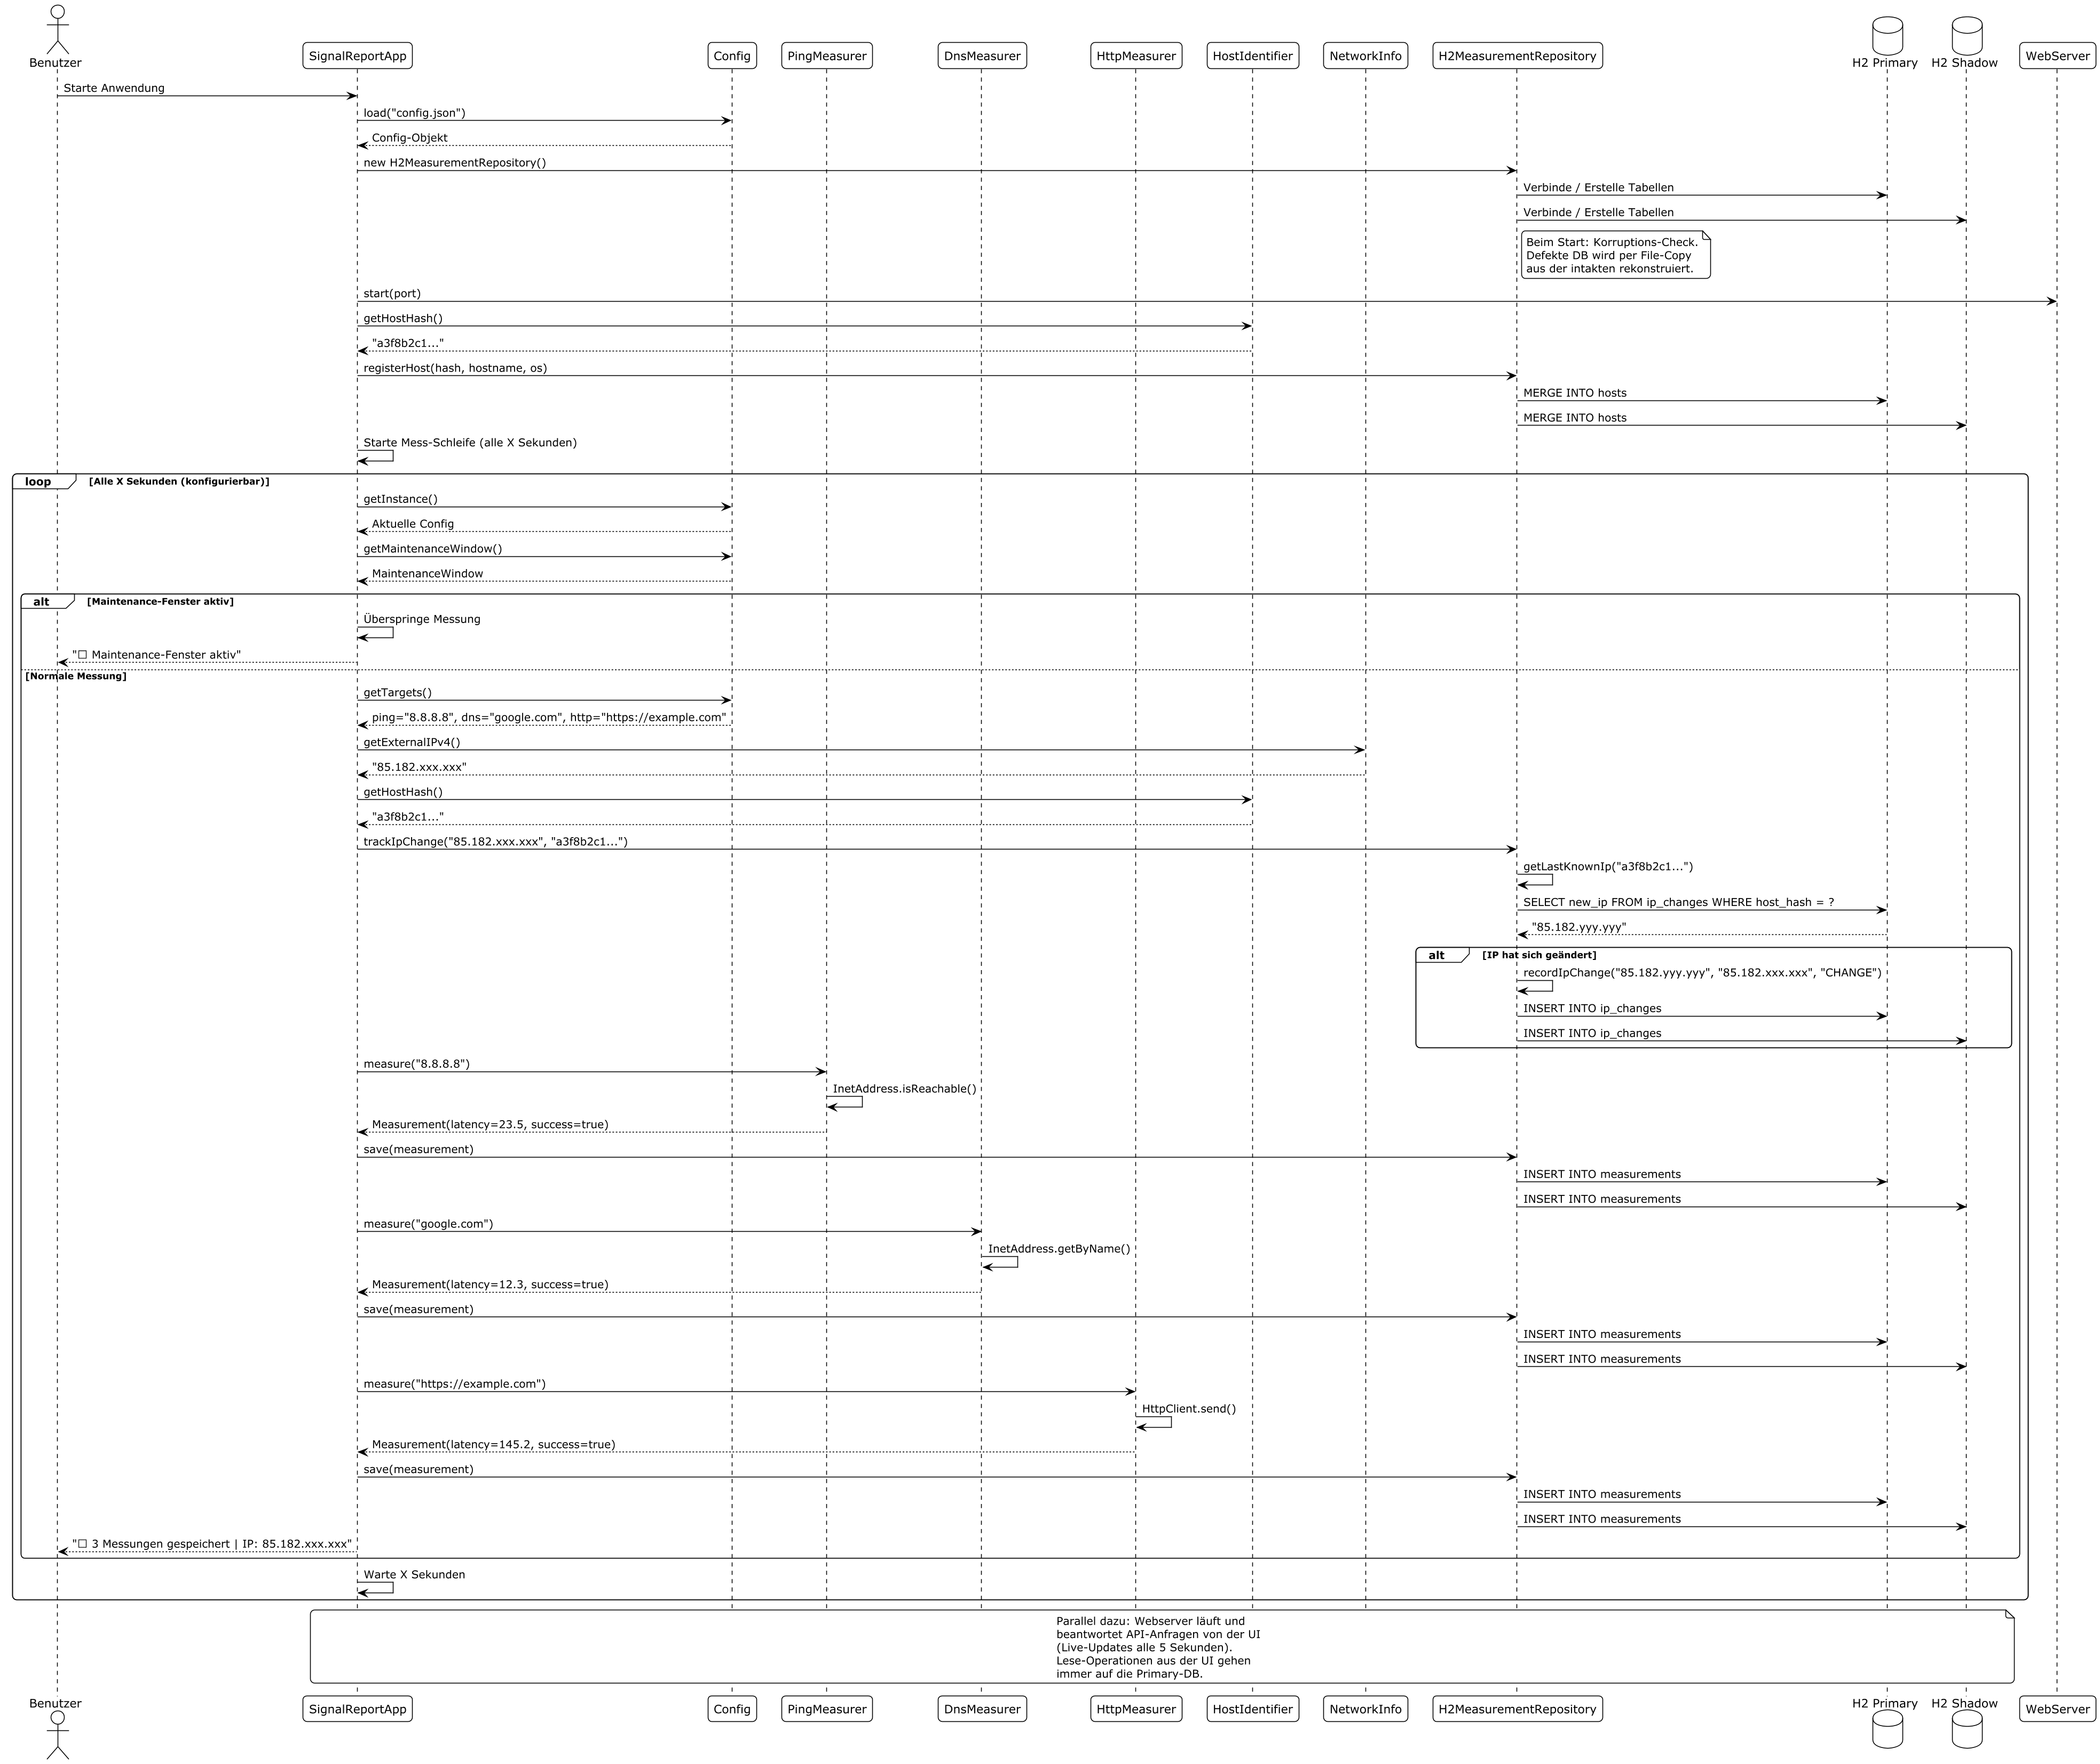
\includegraphics[width=\textwidth]{../diagrams/sequence-measurement.png}
    \caption{Sequenzdiagramm: Messablauf}
    \label{fig:sequence-measurement}
\end{figure}

\subsection{PDF-Export-Prozess}

Der PDF-Bericht (Abbildung \ref{fig:sequence-pdf}) durchläuft mehrere Schritte:
Statistik-Berechnung, Chart-Generierung mit JFreeChart, Zieländerungs-Erkennung,
Ausfall-Analyse und abschliessende PDF-Zusammenstellung mit OpenPDF.

\begin{figure}[H]
    \centering
    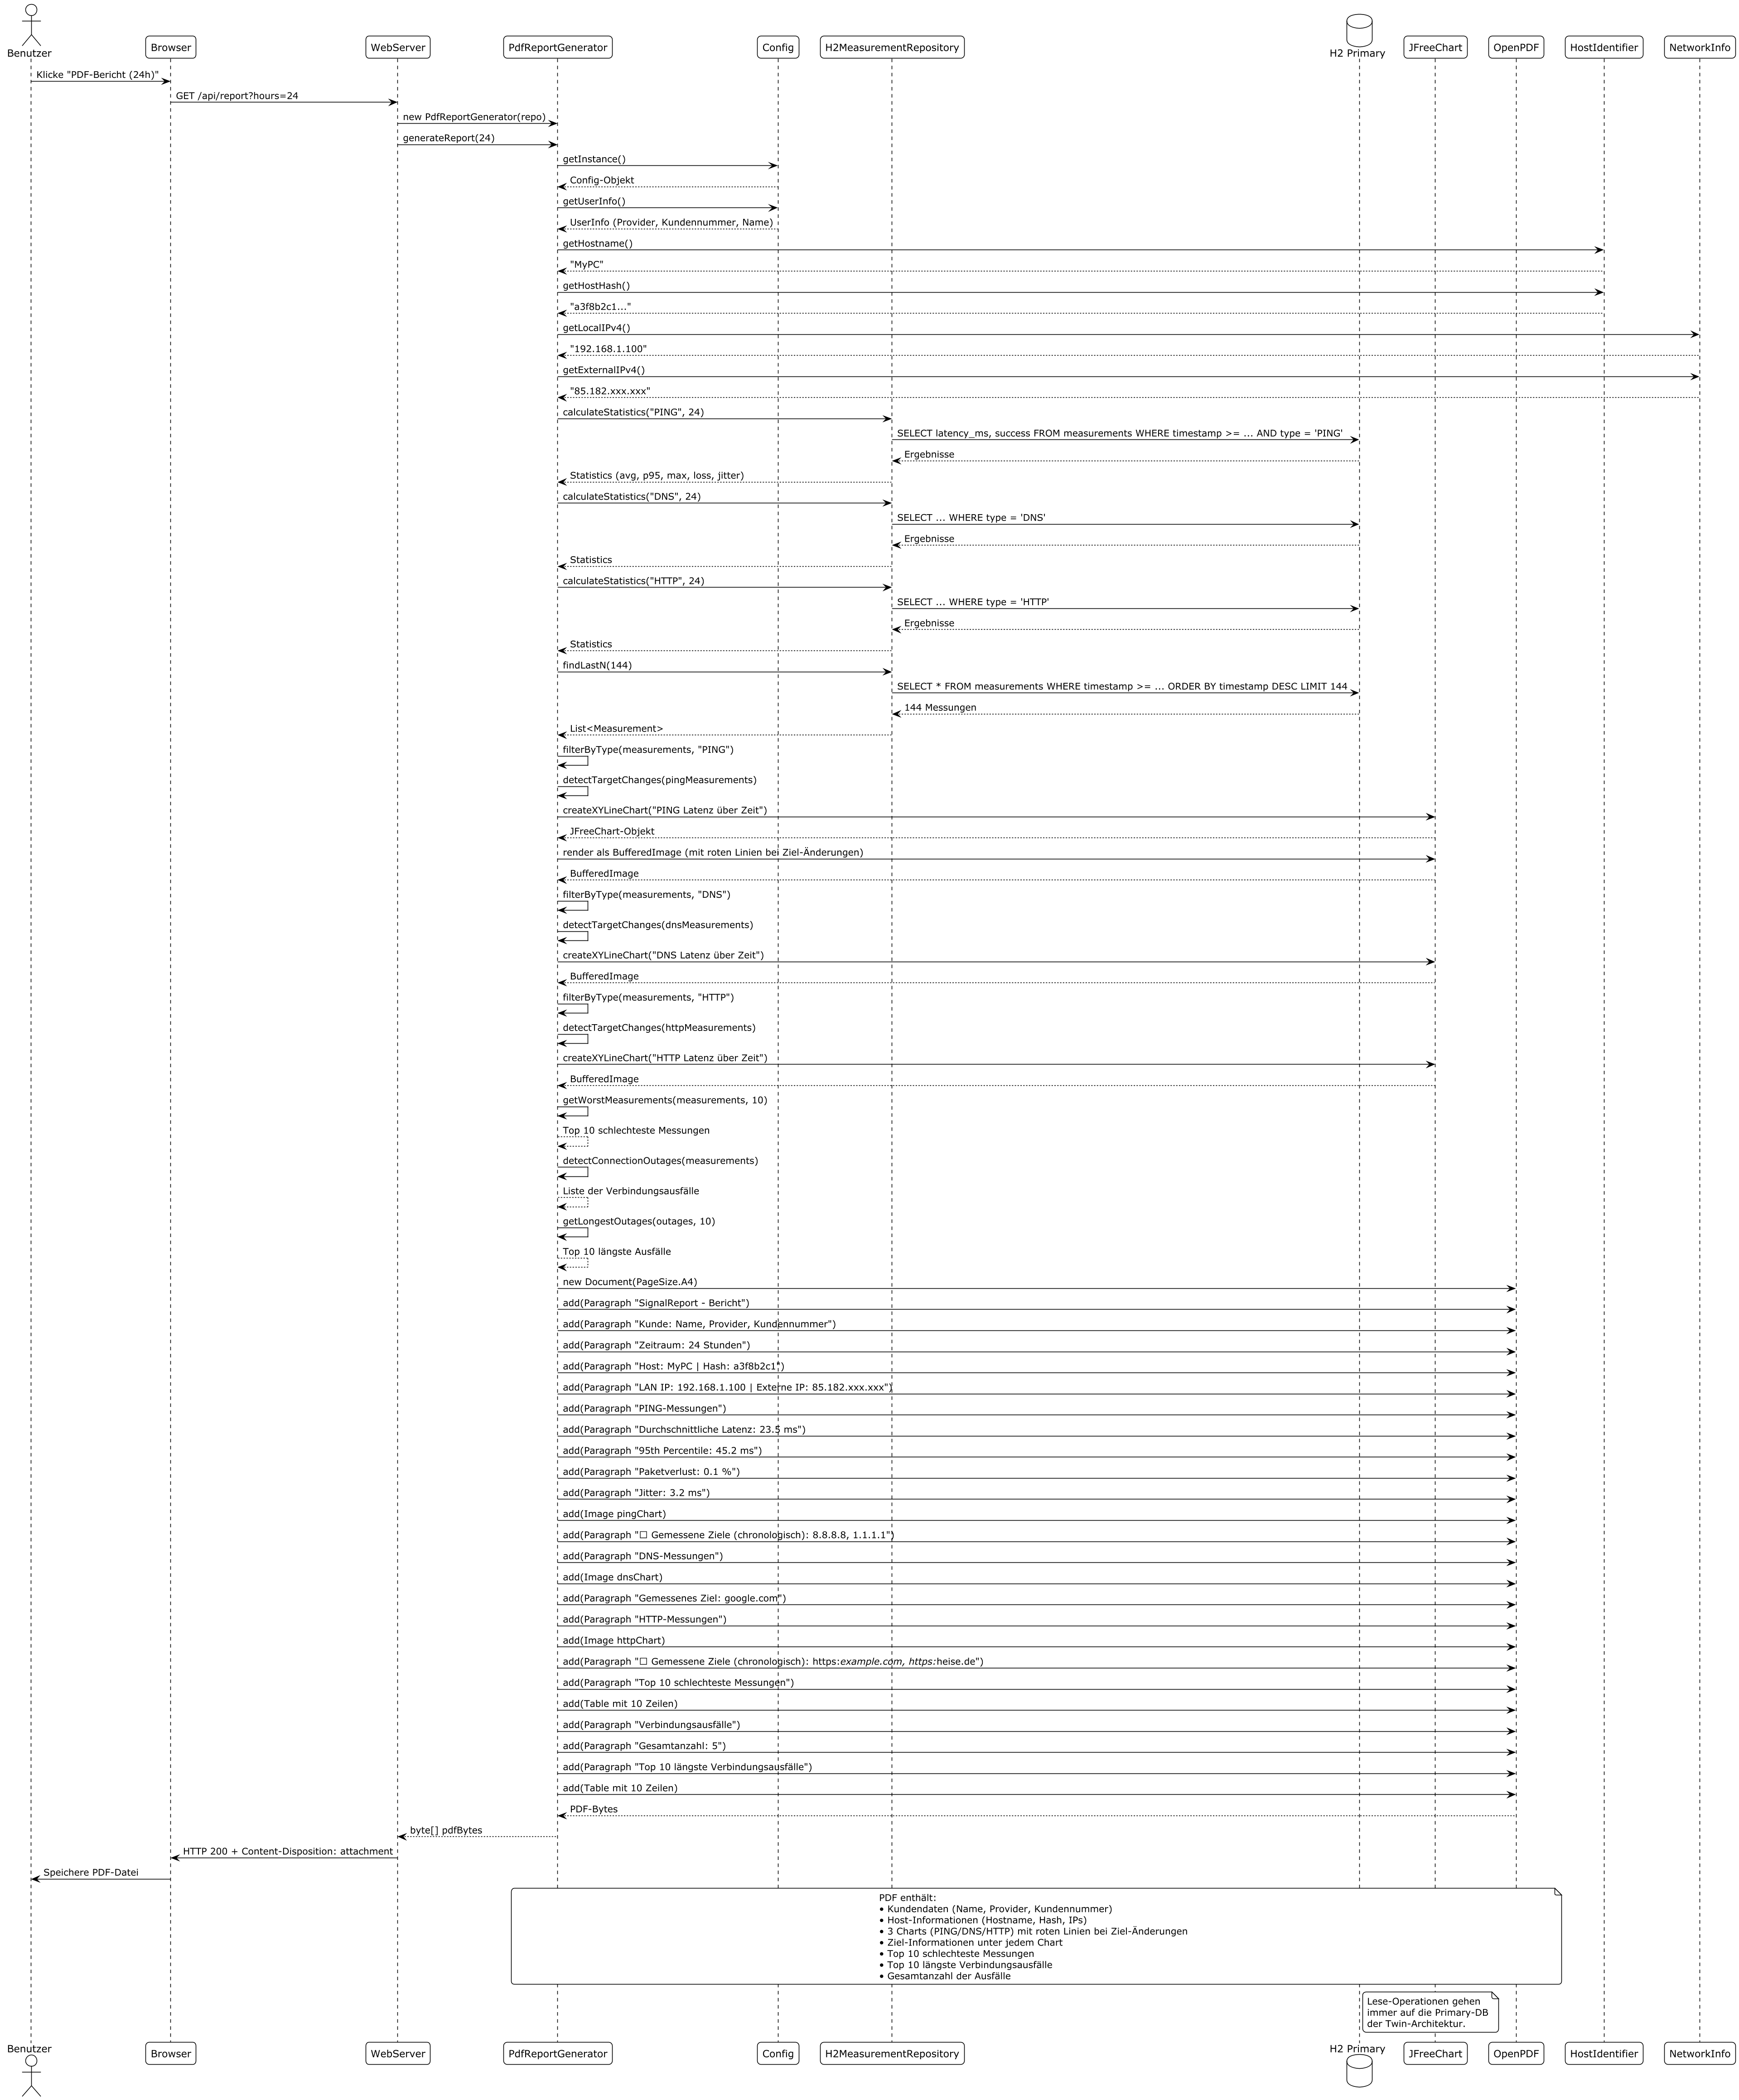
\includegraphics[width=\textwidth]{../diagrams/sequence-pdf.png}
    \caption{Sequenzdiagramm: PDF-Export}
    \label{fig:sequence-pdf}
\end{figure}

\subsection{Use-Cases}

Das Use-Case-Diagramm (Abbildung \ref{fig:usecase}) zeigt alle 16 Anwendungsfälle,
aufgeteilt auf die drei Akteure Benutzer, Administrator und System. Die vollständigen
User Stories zu jedem Use Case finden sich in Abschnitt \ref{sec:userstories}.

\begin{figure}[H]
    \centering
    
\includegraphics[width=0.9\textwidth]{../diagrams/usecase-diagram.png}
    \caption{Use-Case-Diagramm von SignalReport}
    \label{fig:usecase}
\end{figure}

\subsection{Authentifizierungs-Zustände}

Das State-Diagramm (Abbildung \ref{fig:state-auth}) modelliert den Lebenszyklus der
Authentifizierung: vom initialen Setup über den öffentlichen Zugriff bis zum geschützten
Modus mit Admin- und User-Rollen.

\begin{figure}[H]
    \centering
    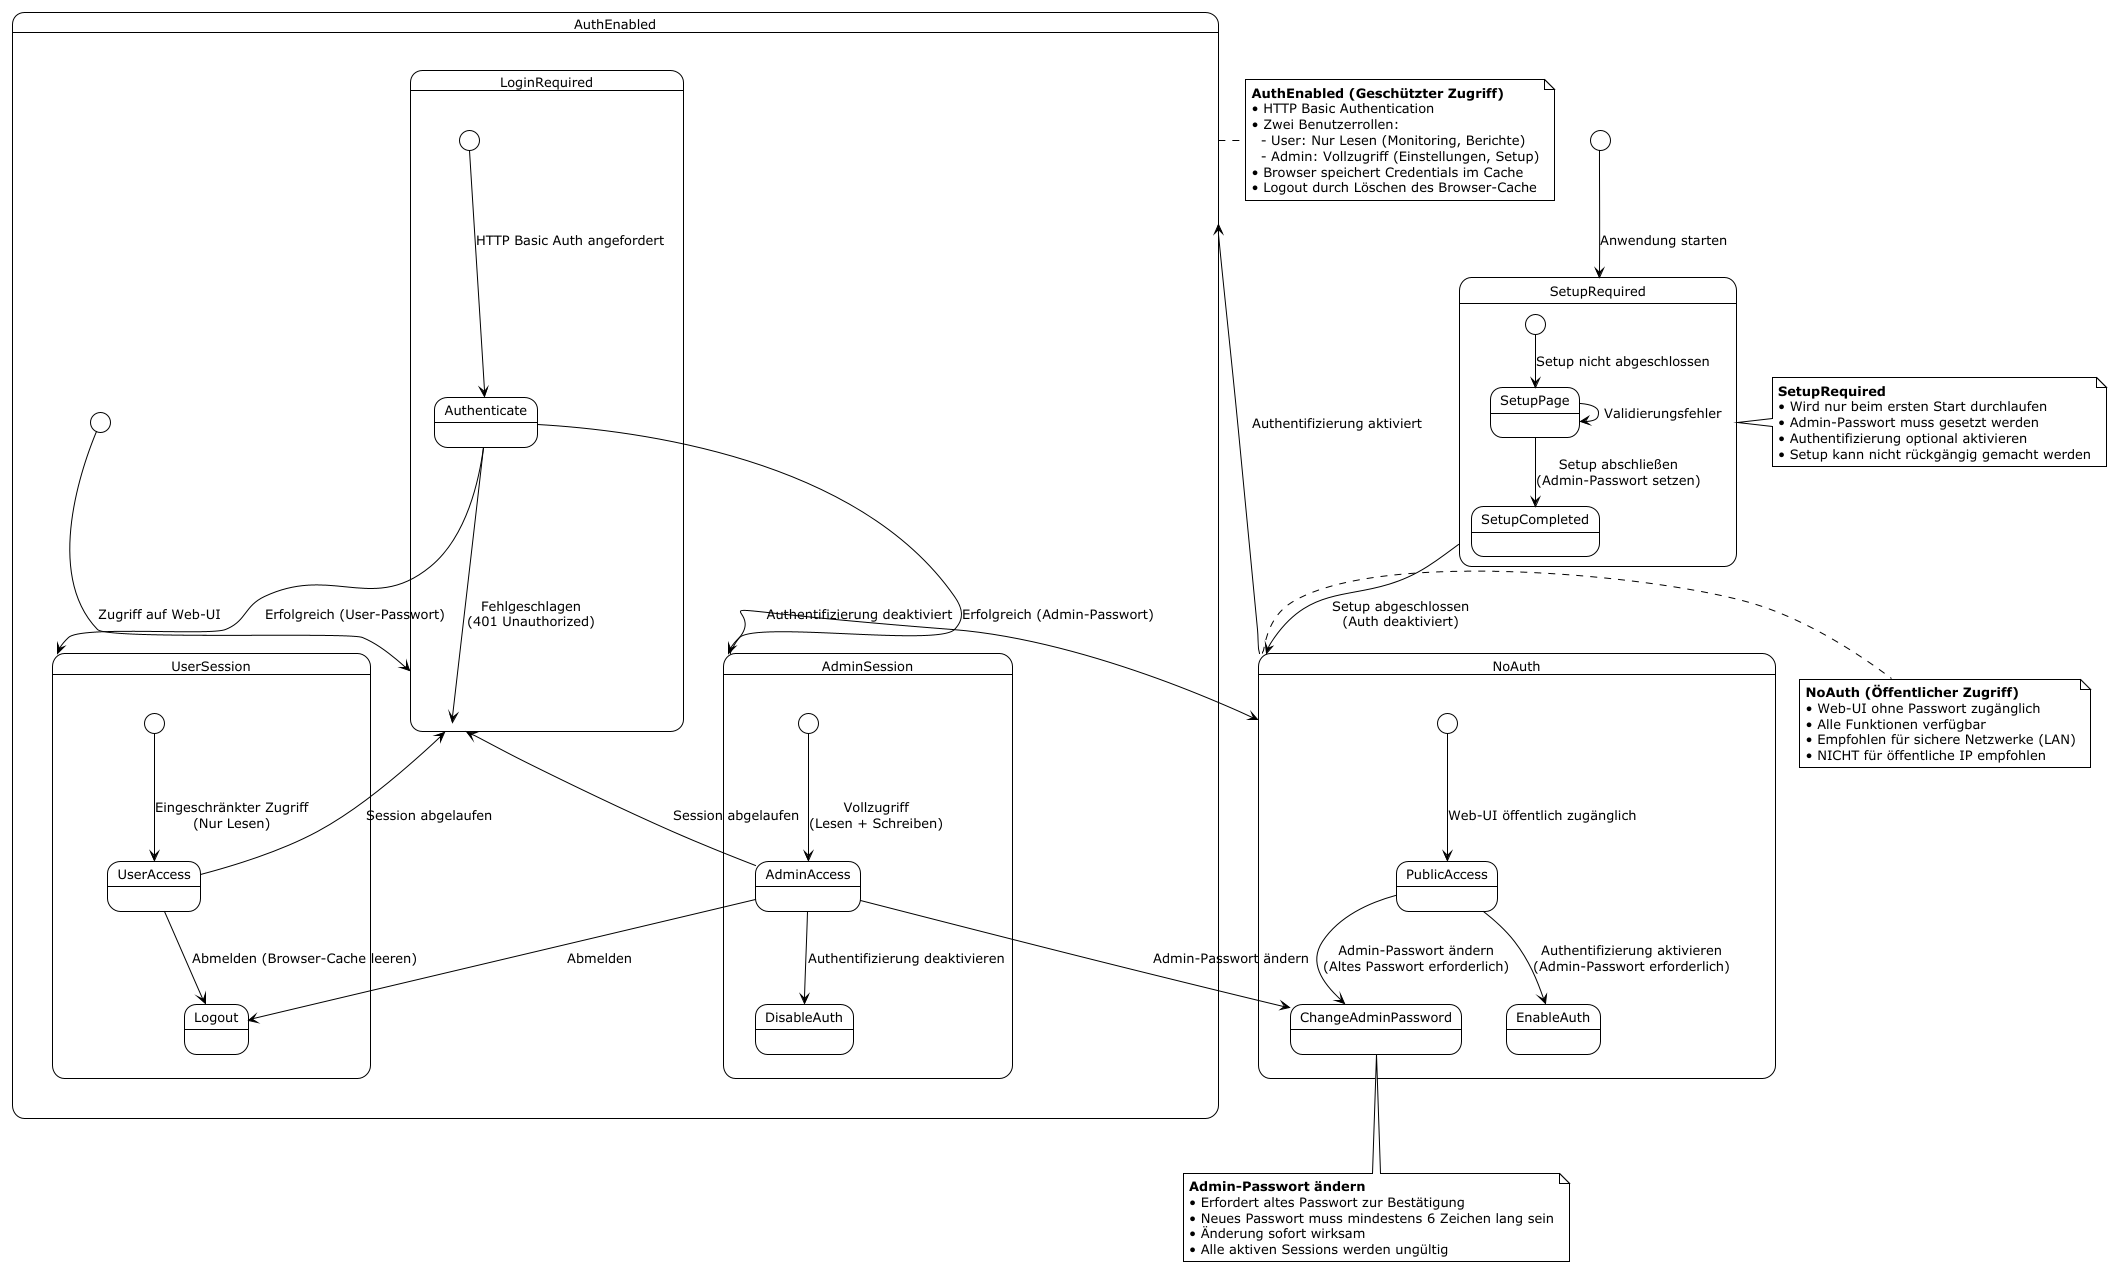
\includegraphics[width=0.9\textwidth]{../diagrams/state-diagram-auth.png}
    \caption{State-Diagramm: Authentifizierung}
    \label{fig:state-auth}
\end{figure}
